%section{7.11.3}%section{7.11.4}%7.11.2-3-4 gir ett plott.
Vi plotter responsen $\frac{|\xi|}{A}$ på tre måter. Først som en funksjon av frekvensen. Så, funnet ved Froude-Krylov-approksimasjonen $X_2^{FK}$, der $b_{22}$ finnes ved Haskind-relasjonene, og der effekten av addert masse $a_{22}$ er ignorert. Og til slutt, approksimasjonen, men justert for addert masse. Vi ser at verdiene for resonansfrekvensen tilsvarer toppene på kurvene våre.

\noindent
\begin{minipage}[t]{0.45\linewidth}
    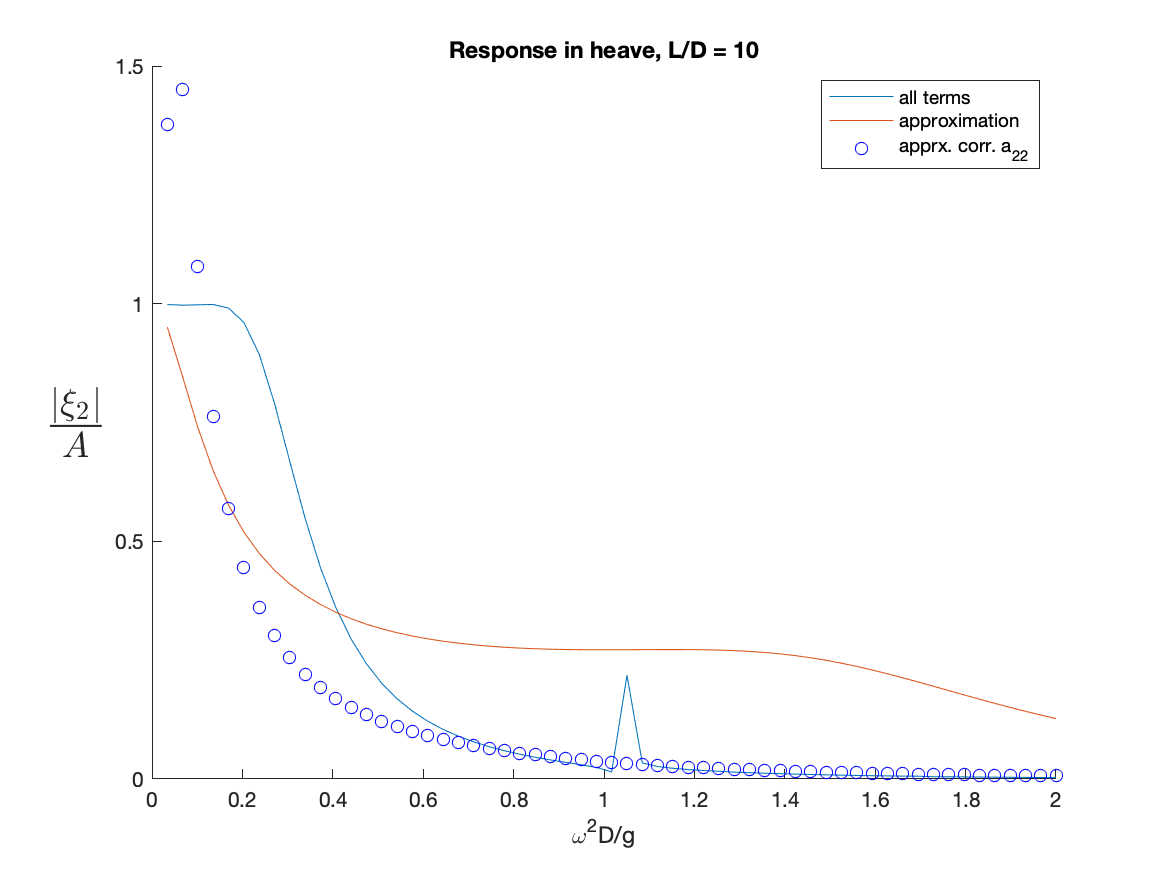
\includegraphics[width=\linewidth]{/Users/ole/Tex/MEK4420/oblig2images/rao_plot1_LD_1.png}
    \captionof{figure}{L/D = 10}
\end{minipage}
\hspace{0.05\linewidth}
\begin{minipage}[t]{0.45\linewidth}
    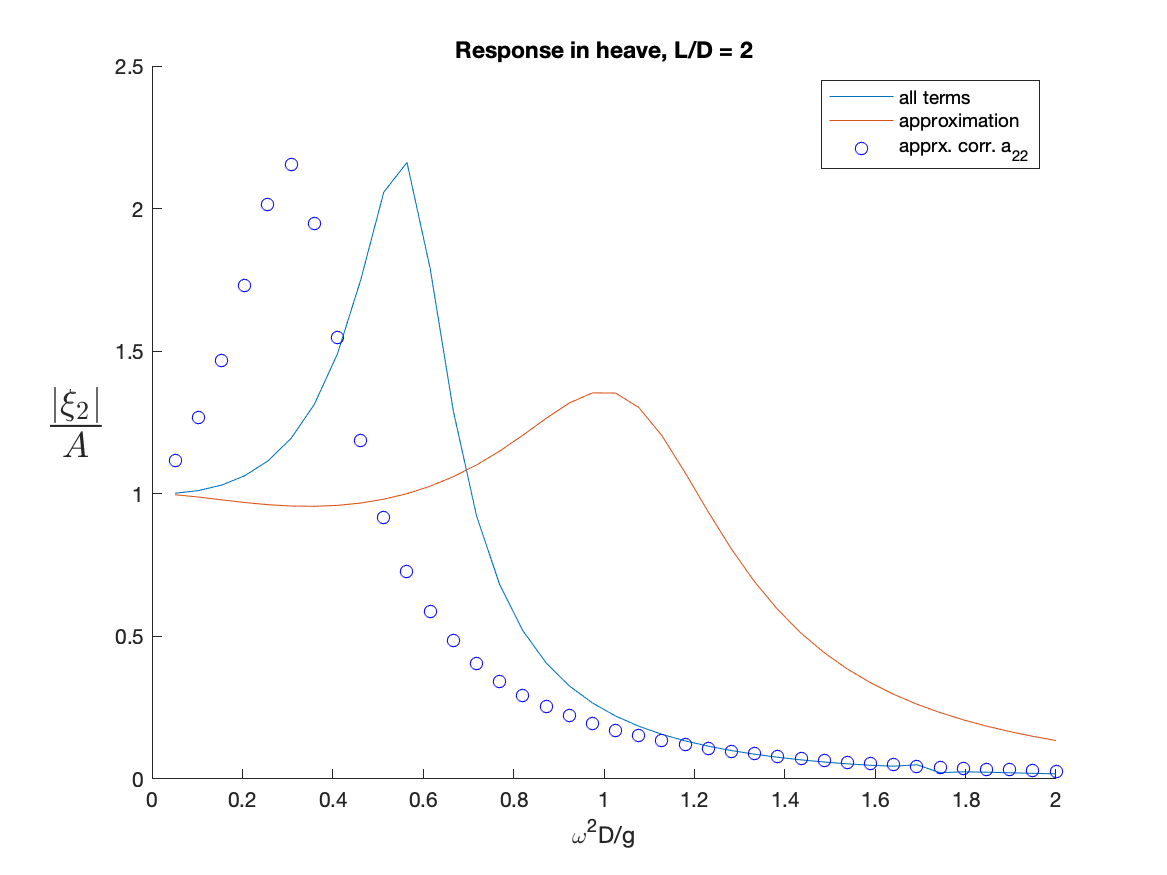
\includegraphics[width=\linewidth]{/Users/ole/Tex/MEK4420/oblig2images/rao_plot2_LD_2.png}
    \captionof{figure}{L/D = 2}
\end{minipage}

\vspace{0.5cm} % Adds vertical space between rows

\noindent
\begin{minipage}[t]{0.45\linewidth}
    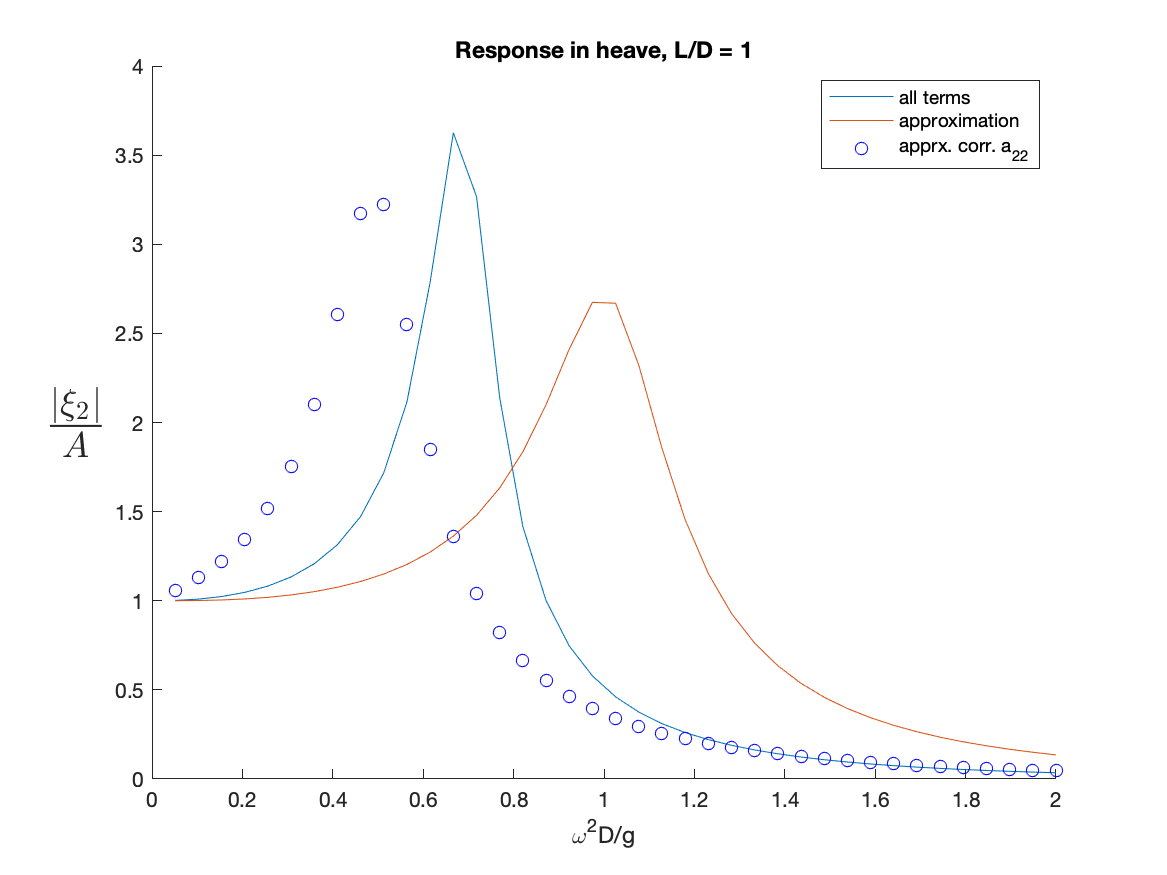
\includegraphics[width=\linewidth]{/Users/ole/Tex/MEK4420/oblig2images/rao_plot3_LD_3.png}
    \captionof{figure}{L/D = 1}
\end{minipage}
\hspace{0.05\linewidth}
\begin{minipage}[t]{0.45\linewidth}
    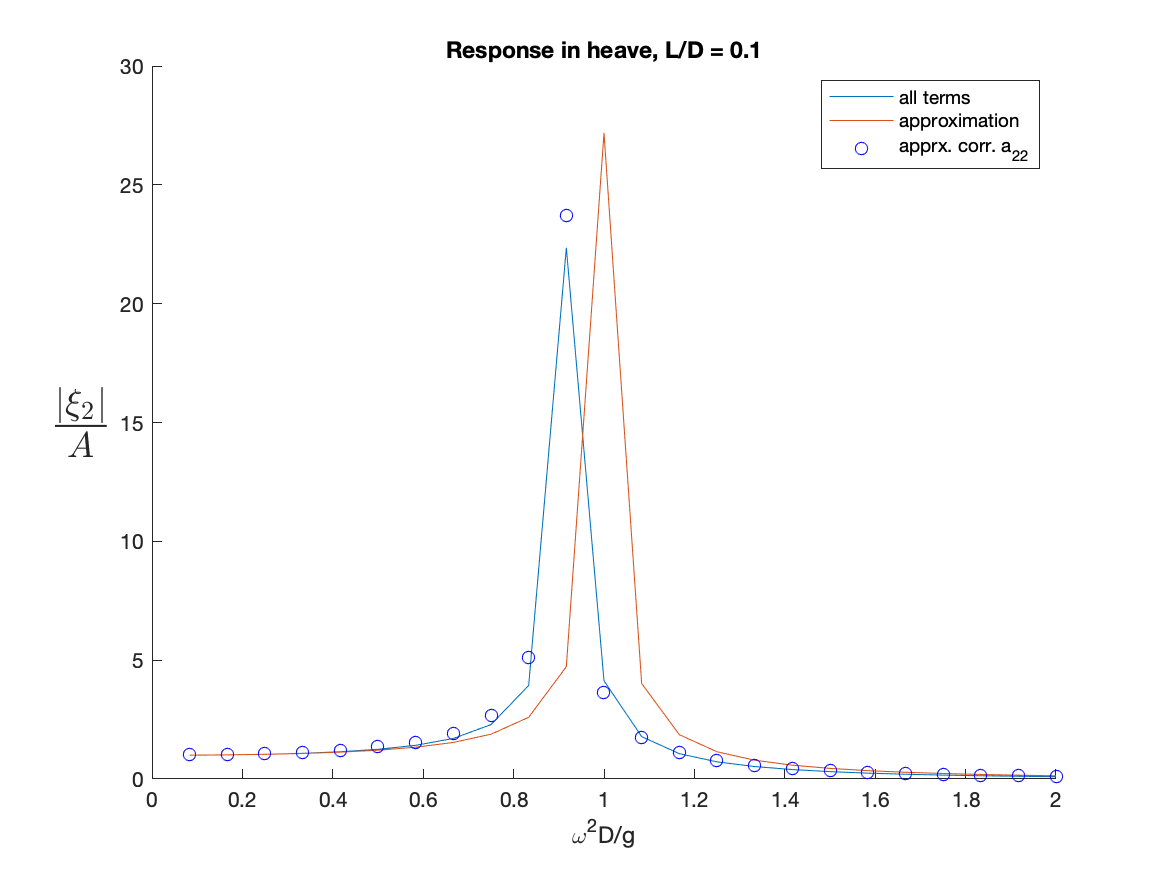
\includegraphics[width=\linewidth]{/Users/ole/Tex/MEK4420/oblig2images/rao_plot4_LD_4.png}
    \captionof{figure}{L/D = 0.1}
\end{minipage}